%%%%%%%%%%%%%%%%%%%%%%%%%%%%%%
%
%		Master thesis report
% 	Visualisation of Gene Ontology and Cluster Analysis Results
%	Author: Vladyslav Aleksakhin

\documentclass[a4paper,oneside]{article}

\usepackage{tabularx}
\usepackage{graphicx}
\usepackage{url}
\usepackage{color}
\usepackage{listings}


\newcommand*{\mywebref}[3]{
	\bibitem{#1} #2 is available on the web \url{#3}. Last access in September 2010.
}

\newcommand*{\todo}[1]{
	\begin{LARGE}
		\textcolor{red}{#1}
	\end{LARGE}
}
 
\begin{document}

\begin{titlepage}
\begin{center}

\Huge{Visualisation of Gene Ontology and Cluster Analysis Results}

\vfill

\begin{Large}
Master's Thesis Report (30 credit points)

\vfill

Supervisor: Prof. Dr. Andreas Kerren\\
Student: Vladyslav Aleksakhin

\vfill

Linneuniversitetet\\
School of Computer Science, Physics and Mathematics

\end{Large}


\end{center}
\end{titlepage}

\tableofcontents
\newpage

\section*{Abstract}
\addcontentsline{toc}{section}{Abstract}

\newpage

\section*{Acknowledgements}
\addcontentsline{toc}{section}{Acknowledgements}

\section{Introduction}
\label{introduction}
\subsection{Motivation}

\subsection{Purpose}

\subsection{Report structure}
Section~\ref{introduction} presents the results of the literature review, where been exploring relevant research efforts in the fields of Bioinformatic, Information and Bio Visualization, in connection to the work. In Section~\ref{problem_statement_and_goals} explains the problem and purpose of this work. Section is split in several parts which covers topics: thesis purpose and collaboration, visualisation complexity and goals, description of the input data, data format overview, overview of different graph file formats. In this section, Problem Statement and Goals, have determined the requirements, use cases, and proposed the architecture for thesis application. In Section~\ref{}, 


we describe possible scenarios to identify the features of the envisioned system.  Chapter 6 consists of the initial ideas and interactions we had for our GUI. Chapter 7 is about the technical approach of our application. In that chapter, we describe the visualization techniques, the tag clouds, the clustering algorithm that we have chosen, and the interaction techniques that we have used for having a robust and flexible geovisualization system for visualizing notes and their content. In Chapter 8, we give some explanation about technologies that we have used, and explained the classes that we implemented. In the next chapter (Case Study), we used the first imagined scenario based on what we presented in Chapter 4 and tested it with the application we have implemented. Finally, in Chapter 10 we give our conclusions and we present future work that can help our system to deliver better results.

\subsection{Information Visualization}

\subsection{Bioinformatic}
\label{bioinformatic}

"In the last few decades, advances in molecular biology and the equipment available for research in this field have allowed the increasingly rapid sequencing of large portions of the genomes of several species. In fact, to date, several bacterial genomes, as well as those of some simple eukaryotes (e.g., Saccharomyces cerevisiae, or baker's yeast) have been sequenced in full. The Human Genome Project, designed to sequence all 24 of the human chromosomes, is also progressing. Popular sequence databases, such as GenBank and EMBL, have been growing at exponential rates. This deluge of information has necessitated the careful storage, organization and indexing of sequence information. Information science has been applied to biology to produce the field called Bioinformatics.


The simplest tasks used in bioinformatics concern the creation and maintenance of databases of biological information. Nucleic acid sequences (and the protein sequences derived from them) comprise the majority of such databases. While the storage and or organization of millions of nucleotides is far from trivial, designing a database and developing an interface whereby researchers can both access existing information and submit new entries is only the beginning. The most pressing tasks in bioinformatics involve the analysis of sequence information"~\cite{Biology}


Here we can find short introduction and history of Bioinformatics: "Bioinformatics is the application of information technology to the field of molecular biology. The term bioinformatics was coined by Paulien Hogeweg in 1978 for the study of informatic processes in biotic systems. Bioinformatics now entails the creation and advancement of databases, algorithms, computational and statistical techniques, and theory to solve formal and practical problems arising from the management and analysis of biological data. Over the past few decades rapid developments in genomic and other molecular research technologies and developments in information technologies have combined to produce a tremendous amount of information related to molecular biology. It is the name given to these mathematical and computing approaches used to glean understanding of biological processes. Common activities in bioinformatics include mapping and analysing DNA and protein sequences, aligning different DNA and protein sequences to compare them and creating and viewing 3-D models of protein structures."~\cite{Bioinformatic}
The primary goal of bioinformatics is to increase our understanding of biological processes. What sets it apart from other approaches, however, is its focus on developing and applying computationally intensive techniques (e.g., data mining, machine learning algorithms, and visualization) to achieve this goal. Major research efforts in the field include sequence alignment, gene finding, genome assembly, protein structure alignment, protein structure prediction, prediction of gene expression and protein-protein interactions, genome-wide association studies and the modelling of evolution.

\subsection{Gene Ontology}
\label{gene_ontology}

As stated above, there are different knowledge databases for biologic information storage. Gene Ontology~\cite{GO_website} project is one of the first-rate international projects. The Gene Ontology, or GO, is a major bioinformatics initiative to unify the representation of gene and gene product attributes across all species. The aims of the Gene Ontology project are threefold; firstly, to maintain and further develop its controlled vocabulary of gene and gene product attributes; secondly, to annotate genes and gene products, and assimilate and disseminate annotation data; and thirdly, to provide tools to facilitate access to all aspects of the data provided by the Gene Ontology project. The GO is part of a larger classification effort, the Open Biomedical Ontologies (OBO)~\cite{OBO}. The Gene Ontology project provides an ontology of defined terms representing gene product properties. The ontology covers three domains; cellular component, the parts of a cell or its extracellular environment; molecular function, the elemental activities of a gene product at the molecular level, such as binding or catalysis; and biological process, operations or sets of molecular events with a defined beginning and end, pertinent to the functioning of integrated living units: cells, tissues, organs, and organisms. Each GO term within the ontology has a term name, which may be a word or string of words; a unique alphanumeric identifier; a definition with cited sources; and a name space indicating the domain to which it belongs. Terms may also have synonyms, which are classed as being exactly equivalent to the term name, broader, narrower, or related; references to equivalent concepts in other databases; and comments on term meaning or usage. The GO ontology is structured as a directed acyclic graph, and each term has defined relationships to one or more other terms in the same domain, and sometimes to other domains. The GO vocabulary is designed to be species-neutral, and includes terms applicable to prokaryotes and eukaryotes, single and multicellular organisms. The GO ontology is not static, and additions, corrections and alterations are suggested by, and solicited from, members of the research and annotation communities, as well as by those directly involved in the GO project. For example, an annotator may request a specific term to represent a metabolic pathway, or a section of the ontology may be revised with the help of community experts. Suggested edits are reviewed by the ontology editors, and implemented where appropriate.


\subsection{Clustering}
\label{clustering}

"Data clustering (or just clustering), also called cluster analysis, segmentation analysis, taxonomy analysis, or unsupervised classification, is a method of creating groups of objects, or clusters, in such a way that objects in one cluster are very similar and objects in different clusters are quite distinct. Data clustering is often confused with classification, in which objects are assigned to predefined classes. In data clustering, the classes are also to be defined."~\cite{data_clustering_book}


Clustering algorithms can be applied in many fields, for instance:

\begin{itemize}
\item Marketing: finding groups of customers with similar behaviour given a large database of customer data containing their properties and past buying records;
\item Biology: classification of plants and animals given their features;
\item Libraries: book ordering;
\item Insurance: identifying groups of motor insurance policy holders with a high average claim cost; identifying frauds;
\item City-planning: identifying groups of houses according to their house type, value and geographical location;
\item Earthquake studies: clustering observed earthquake epicentres to identify dangerous zones;
\item WWW: document classification; clustering web log data to discover groups of similar access patterns.
\end{itemize}

\section{Problem Statement and Goals}
\label{problem_statement_and_goals}
The aim of the tool is to discover relations in separated datasets (Gene Ontology graph and cluster analysis result tree), visualize and allow interactive selection relations selection.


First step in the program work is loading data and to compute connected components. Data is stored in GML file format. More detailed information about this format and other graph file formats is in the section~\ref{dataset_description}.

Here is program algorithm explanation using sample graphs:
\begin{enumerate}
\item The program visualizes Gene Ontology and cluster analysis result tree. Visualization technic is discussed in the section~\ref{solution}.
\item Interactively select node in the Gene Ontology graph (Figure~\ref{step_1}).

\begin{figure}
	\begin{center}
		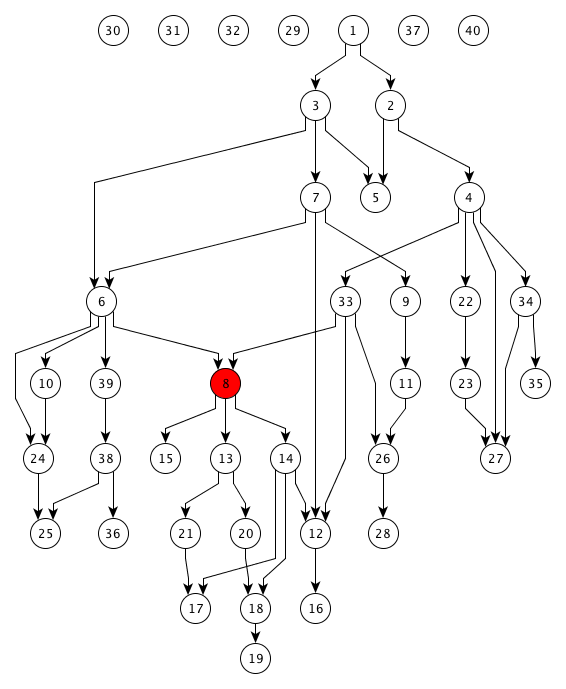
\includegraphics[scale=0.5]{subgraph_extraction_algorithm_step_1.png}
	\end{center}
	\caption{Selected node in the Gene Ontology}
	\label{step_1}
\end{figure}

\item When node is selected in the Gene Ontology program computes all successors (Figure~\ref{step_2}).

\begin{figure}
	\begin{center}
		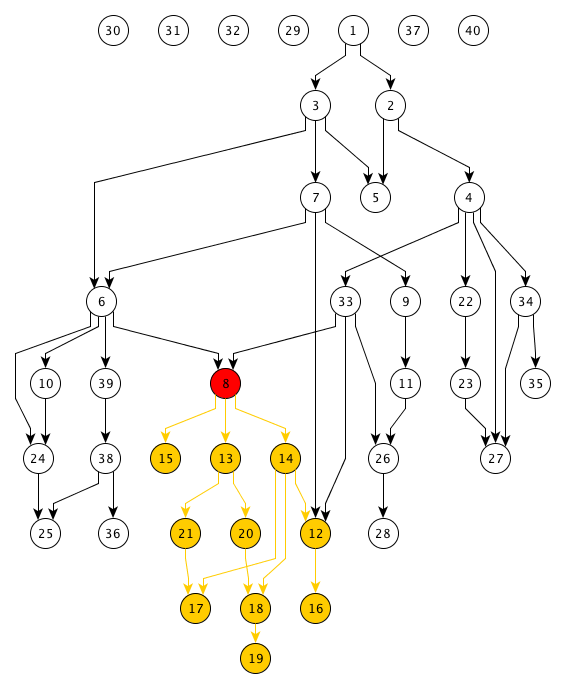
\includegraphics[scale=0.5]{subgraph_extraction_algorithm_step_2.png}
	\end{center}
	\caption{Corresponded successors of the selected node}
	\label{step_2}
\end{figure}


\item Extract leafs from successors (Figure~\ref{step_3}).

\begin{figure}
	\begin{center}
		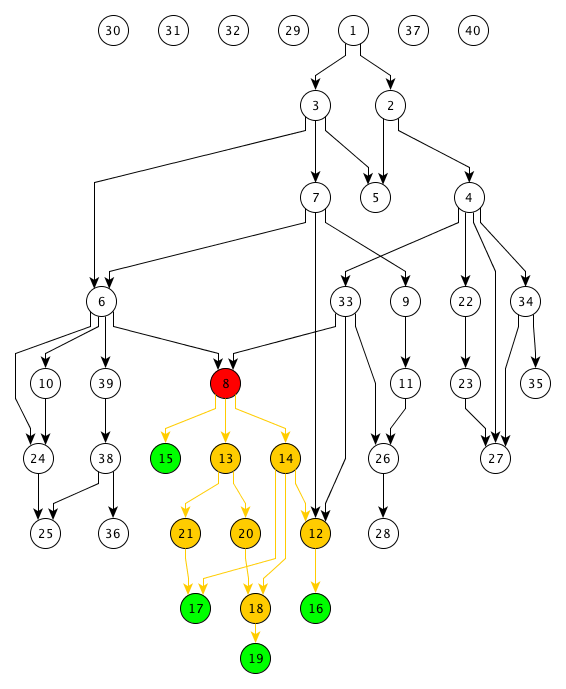
\includegraphics[scale=0.5]{subgraph_extraction_algorithm_step_3.png}
	\end{center}
	\caption{Extract leafs}
	\label{step_3}
\end{figure}


\item Then the program searches corresponded leaves in cluster analysis result tree by label as seen on the Figure~\ref{step_4}.

\begin{figure}
	\begin{center}
		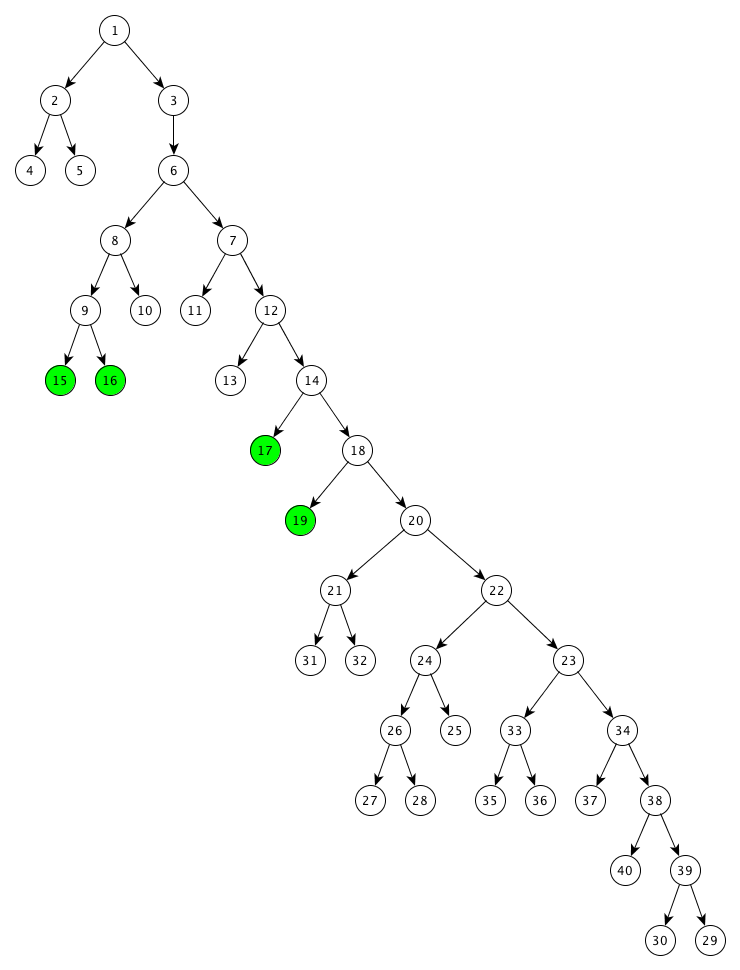
\includegraphics[scale=0.5]{subgraph_extraction_algorithm_step_4.png}
	\end{center}
	\caption{Corresponded leaves in the cluster tree}
	\label{step_4}
\end{figure}

\item For this leaves the program founds root connected to all leaves and extract corresponding sub trees (Figure~\ref{step_5}).

\begin{figure}
	\begin{center}
		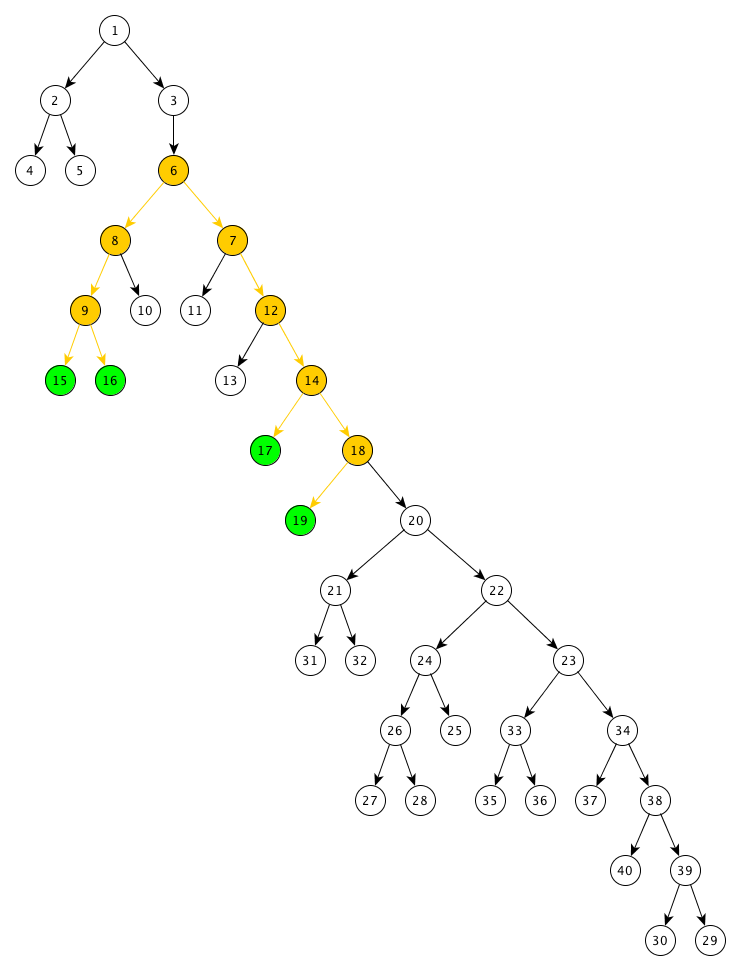
\includegraphics[scale=0.5]{subgraph_extraction_algorithm_step_5.png}
	\end{center}
	\caption{Build sub tree}
	\label{step_5}
\end{figure}


\item Founded sub tree cached. This sub tree is highlighted in cluster analysis tree.
\end{enumerate}
   

\subsection{Thesis Collaboration}
There are many datasets for analysis in biology. This work is intended for making a visualization tool for genes and gene relations, in order to help biologists 
with their work with genes. This project is result of collaboration between ISOVIS research group (Head: Prof. Dr. Andreas Kerren~\cite{Kerren}) of Linneuniversitetet at V\"axj\"o, Sweden, and Plant Bioinformatics Group (Head: Prof. Dr. Falk Schreiber~\cite{Schreiber}) of Leibniz Institute of Plant Genetics and Crop Plant Research (IPK), Germany. 


About the ISOVIS group: "The ISOVIS group mainly focuses on the exploration analysis and visualization of typically large information spaces, for example, in Software Engineering, Geography, or Biology. Another research topic is the use of visualizations in educational software, especially for computer science education. Hereby, we focus on so-called human-centred visualization techniques and approaches:
Human-Centred Visualization combines traditional visualization techniques with the ability of the human visual-brain system and/or the haptic-motoric system to explore and analyse complex data sets comprehensively. This kind of visualization merges several aspects of different research areas, such as Information Visualization, Scientific Visualization, Human-Computer Interaction, Data Mining, Information Design, Graph Drawing, and Computer Graphics. From all sub fields in visualization, we mainly focus on Information Visualization which centres on the visualization of abstract data, e.g., hierarchical, networked, or symbolic information sources, in order to help users understand and analyse such data.


For most practical applications, researchers try to find the best visual representation of the given information. That is the core problem of each visualization but sometimes the seemingly best representation does not suffice if the human information processing and the human capability of information reception are not adequately taken into account. Additionally, these aspects depend on the data to be visualized and on the user's background. While the development of human-centred visualization tools, user abilities and requirements, visualization tasks, tool functions, and visual representations should be equally taken into account. The design of such tools is one of the large challenges of Information Visualization, Software Visualization, and of many application areas, such as the visualization of biological/biochemical or geographical information."~\cite{ISOVIS}


As said on official page of Plant Bioinformatic Group: ”The research group focuses on modelling, analysis, simulation and visualisation of biological networks in the context of plant biological problems. Our aim is the development of methods and software tools for the analysis of complex biological networks. Therefore we integrate, process and analyse data from different areas of genome, proteome and 
metabolome research and present the results in a user-friendly way. The emphasis is on the linkage of experimental data about expression profiles and metabo- 
lite patterns with metabolic and regulatory networks. The data and complex connections are modelled using graphs. We are developing graph (network) analysis and interactive visualisation methods to discover network properties and to make the data easily accessible to the user. A subsequent step is to use the data for the simulation of metabolic and regulatory networks.”~\cite{PBG}


\subsection{Dataset Description}
\label{dataset_description}
Gene Ontology data and cluster analysis results presented as directed graphs. They are stored in separate files in special format -- GML files. GML file format covered in the next section.


GO graph is directed acyclic graph has 10042 vertices and  24155 edges. It has 1 root, 2729 nodes and 7312 leafs (terminal nodes). In the Figure~\ref{yEd_GO} showed visualization of the Gene Ontology graph using yEd~\cite{yed} graph editor using Hierarchical layout. It is obviously shows imperfectness of classic visualization of the graphs.


\begin{figure}[h]
\begin{center}
	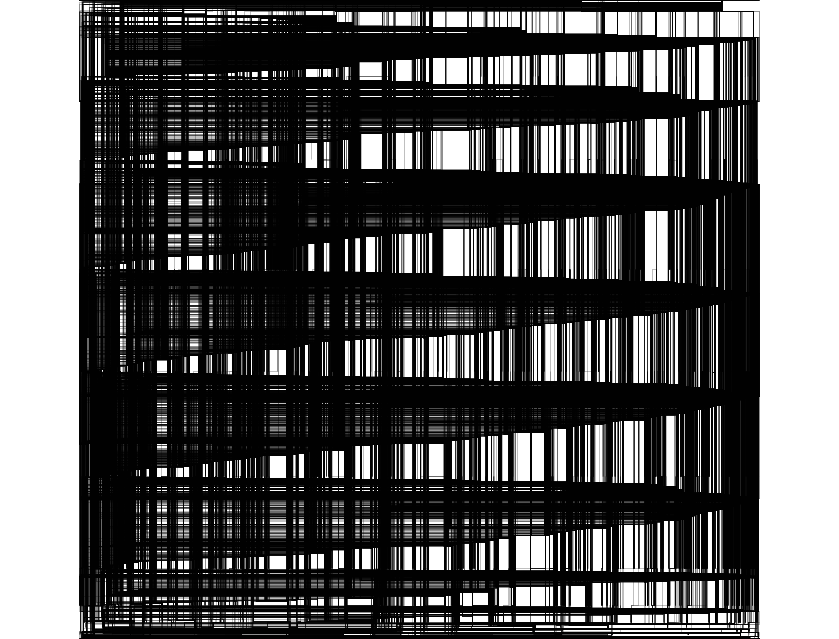
\includegraphics[scale=0.3]{yEd_GO.png}
	\label{yEd_GO}
	\caption{Gene Ontology yEd visualization}
\end{center}
\end{figure}


Cluster graph is directed binary  tree has 14623 nodes and 14622. Cluster graph as a tree has 1 root, 7310 nodes and 7312 leafs. To get an impression of the graph on the Figure~\ref{Cytoscape_Cluster_1} is visualization of the cluster tree using Cytoscape~\cite{Cytoscape} visualization tool.

\begin{figure}[h]
\begin{center}
	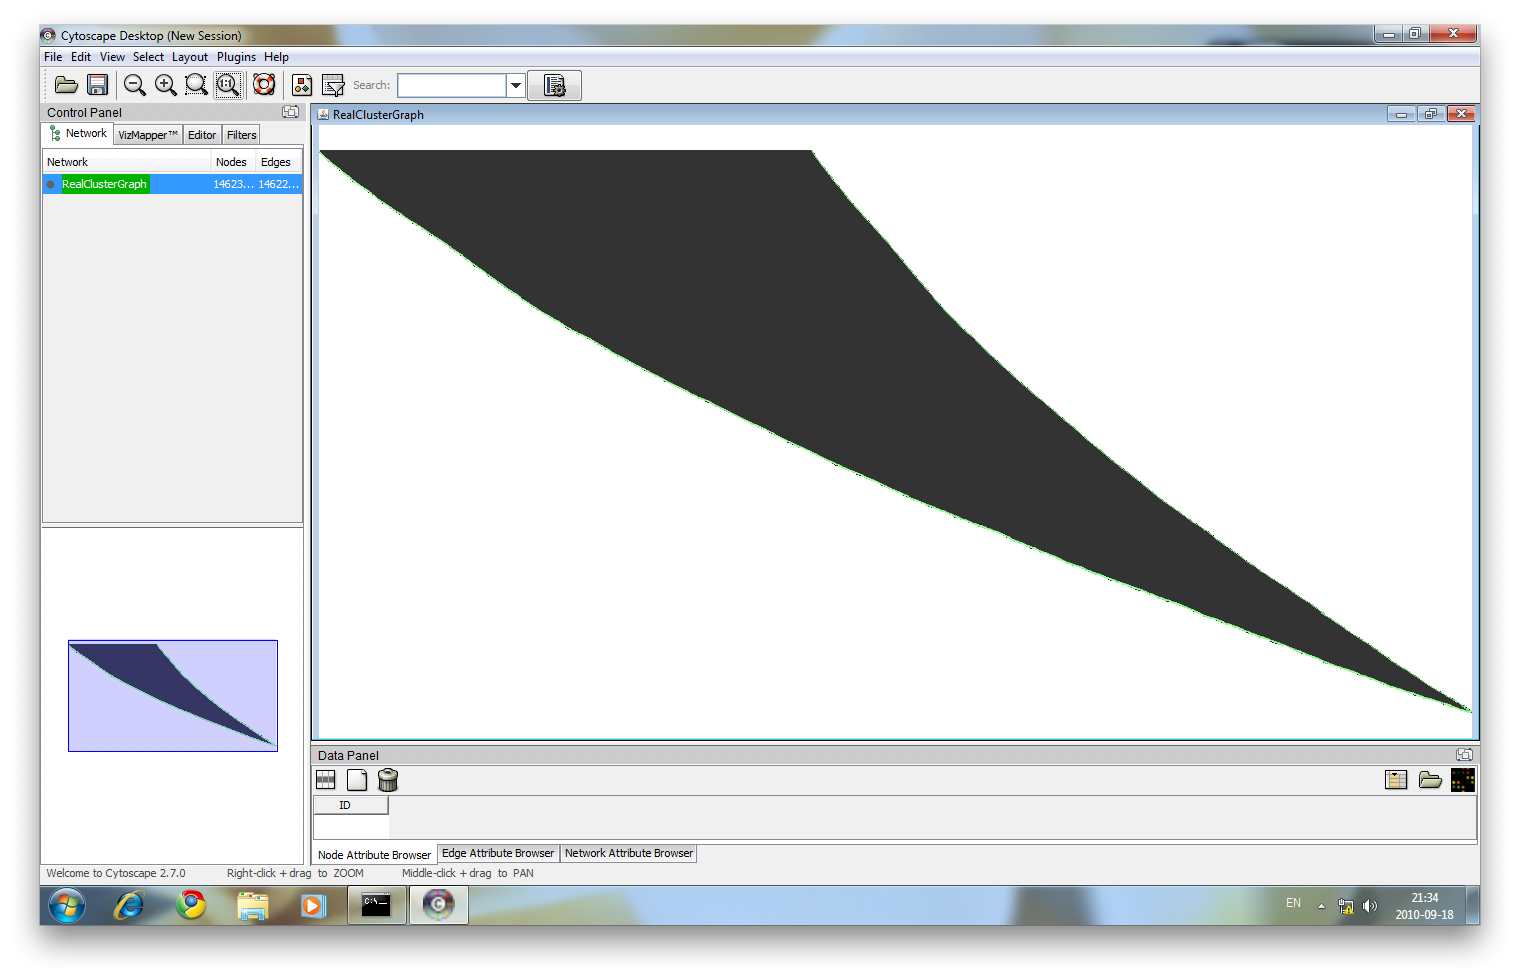
\includegraphics[scale=0.3]{Cytoscape_cluster_graph_1.png}
	\label{Cytoscape_Cluster_1}
	\caption{Cluster analysis result tree Cytoscape visualization tool}
\end{center}
\end{figure}

\begin{figure}[h]
\begin{center}
	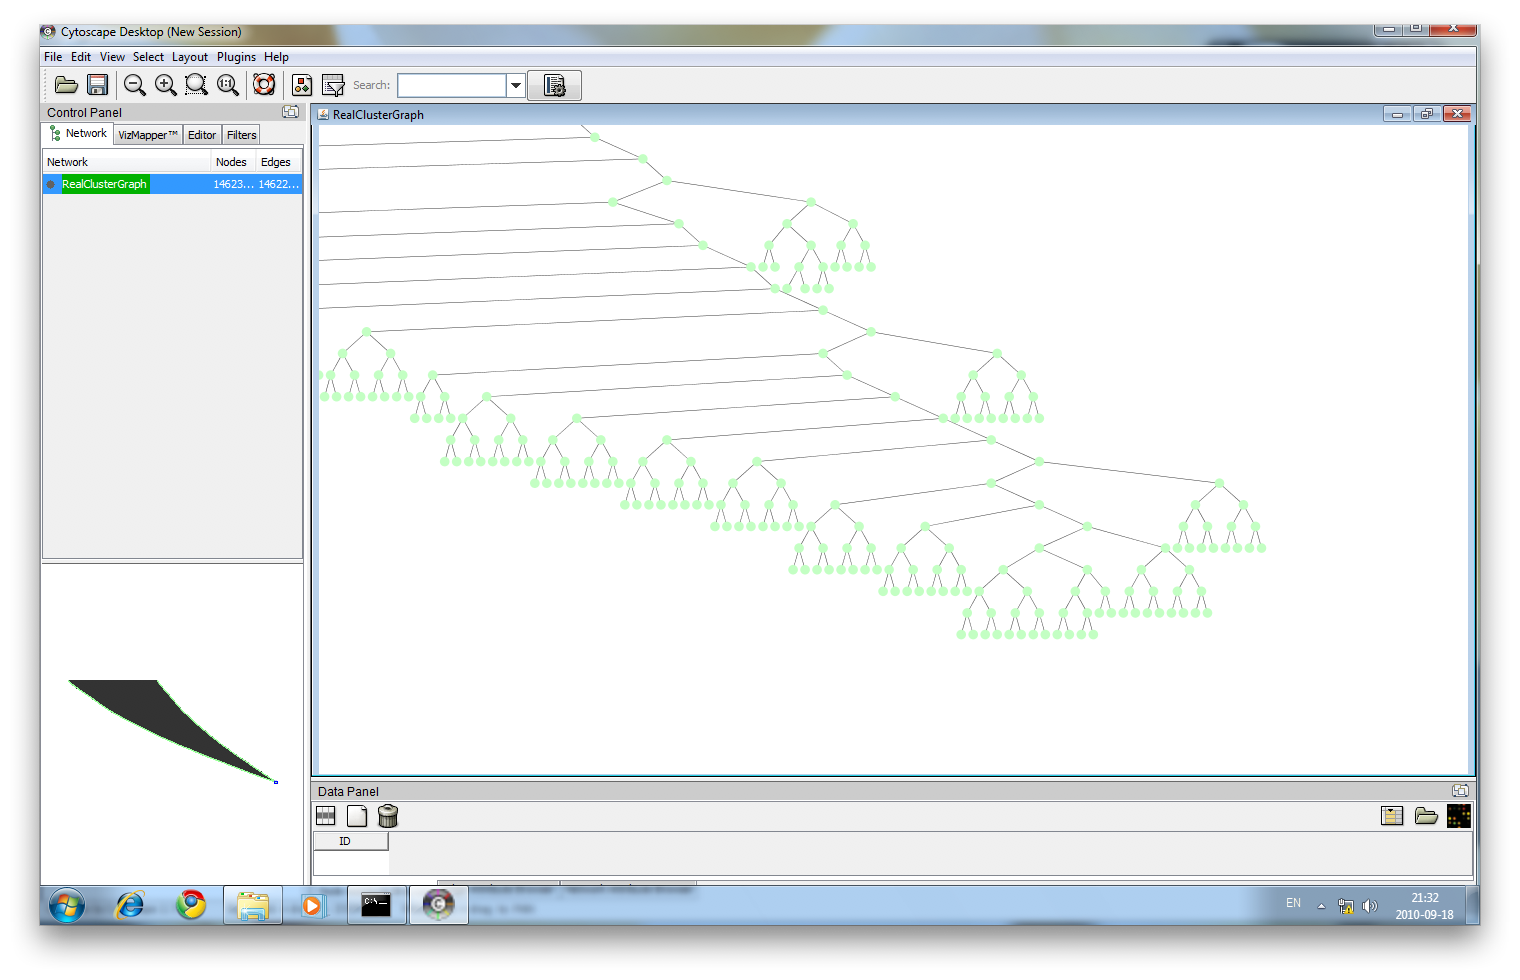
\includegraphics[scale=0.3]{Cytoscape_cluster_graph_2.png}
	\label{Cytoscape_Cluster_2}
	\caption{Zoomed cluster analysis result tree}
\end{center}
\end{figure}

Both of two graphs are independent from each other from developer point of view: they have different node ids and edge ids. But they are corresponded by graph node labels -- both of this graphs have same label for terminal (leaf) graph nodes. This property is used in the sub graph extracting algorithm.


The application should work with large quantity of data over tens of thousands that is why performance is one of the main requirements. It is important to give a consideration on optimization.

\subsection{GML Graph File Format}
 "GML, the Graph Modelling Language, is our proposal for a portable file format for graphs. GML's key features are portability, simple syntax, extensibility and flexibility. A GML file consists of a hierarchical key-value lists. Graphs can be annotated with arbitrary data structures. The idea for a common file format was born at the GD'95; this proposal is the outcome of many discussions. GML is the standard file format in the Graphlet~cite{Graphlet} graph editor system. It has been overtaken and adapted by several other systems for drawing graphs."~\cite{GML}
 
 
GML format is platform independent, and easy to implement. Furthermore, it has the capability to represent arbitrary data structures, since advanced programs have the need to attach their specific data to nodes and edges. GML is flexible enough that a specific order of declarations is not needed, and that any non-essential data may be omitted. Simple graph is showed in the Listing~\ref{sample_graph_gml}

\begin{center}
	\lstinputlisting[language=xml, tabsize=2, caption={GML description of sample graph}, label={sample_graph_gml}]{SampleGraph.gml}
\end{center}

In the Figure~\ref{sample_graph_yed_vis} showed manual visualization of the graph using yEd~\cite{yEd}

\begin{figure}
\begin{center}
	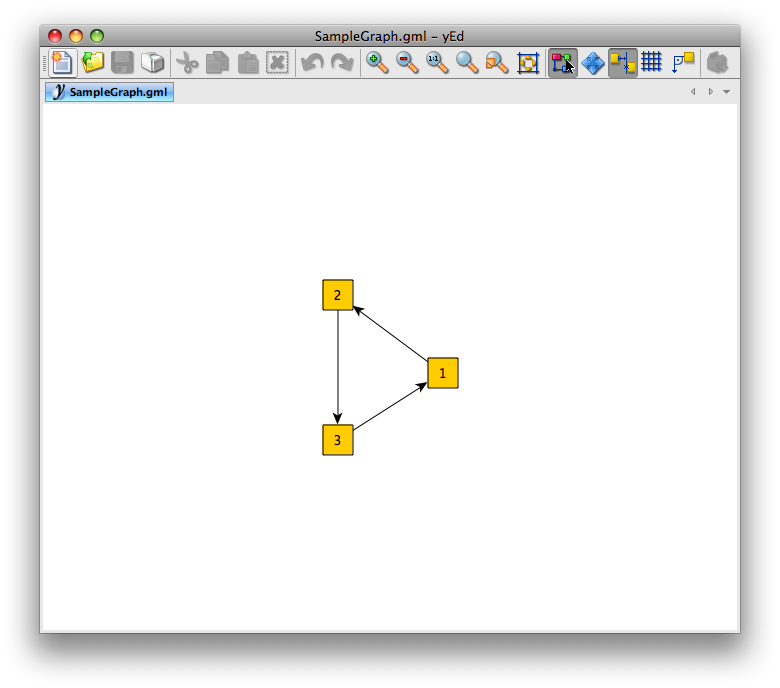
\includegraphics[scale=0.5]{SampleGraph.png}
	\caption{Manual visualization of the sample graph}
	\label{sample_graph_yed_vis}
\end{center}
\end{figure}

More complex graph with additional properties and its visualization produced by yEd graph editor is in the Appendix A and the visualization of this graph showed on the Figure~\ref{yed_graph_vis}

\begin{center}
\begin{figure}
	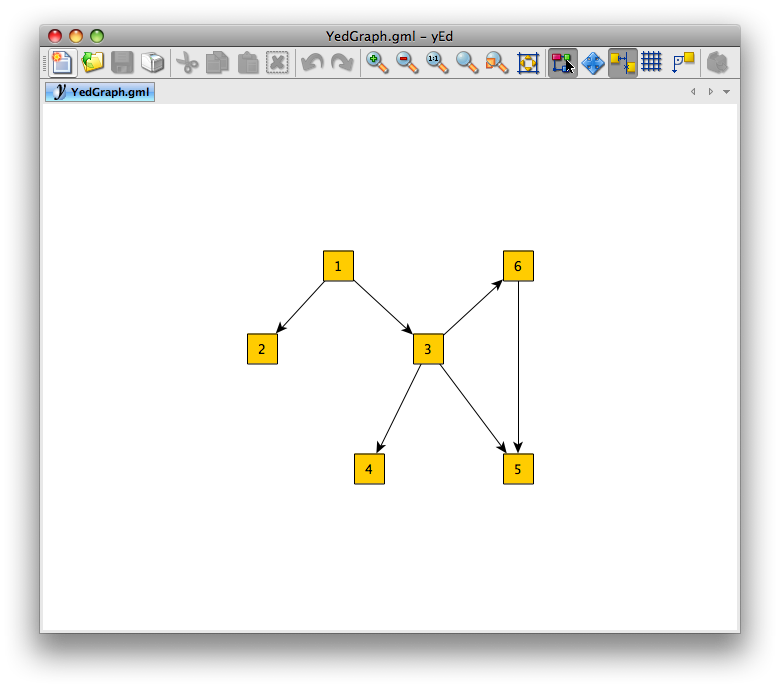
\includegraphics[scale=0.5]{YedGraph.png}
	\caption{Manual visualization of the sample graph}
	\label{yed_graph_vis}
\end{figure}
\end{center}

Applications supporting GML~\cite{GML_wiki}

\begin{itemize}
\item Clairlib~\cite{clairlib}, a suite of open-source Perl modules intended to simplify a number of generic tasks in natural language processing (NLP), information retrieval (IR), and network analysis (NA).
\item Cytoscape~\cite{Cytoscape}, an open source bioinformatics software platform for visualizing molecular interaction networks, loads and save previously-constructed interaction networks in GML.
\item NetworkX~\cite{NetworkX}, an open source Python library for studying complex graphs.
\item ocamlgraph\cite{ocamlgraph}, a graph library for OCaml.
\item OGDF\cite{OGDF}, the Open Graph Drawing Framework, an open source C++ library containing implementations of various graph drawing algorithms. The library is self contained; optionally, additional packages like LP-solvers are required for some implementations.
\item Tulip~\cite{Tulip} (software) is a free software in the domain of information visualisation capable of manipulating huge graphs (with more than 1.000.000 elements).
\item yEd~\cite{yEd}, a free Java-based graph editor, supports import from and export to GML.
\end{itemize}

\subsection{Other Graph File Formats}

\subsubsection{GraphML}
GraphML is a comprehensive and easy-to-use file format for graphs. It consists of a language core to describe the structural properties of a graph and a flexible extension mechanism to add application-specific data.~\cite{GraphML} Its main features include support of:
\begin{itemize}
\item directed, undirected, and mixed graphs;
\item hyper graphs;
\item hierarchical graphs;
\item graphical representations;
\item references to external data;
\item application-specific attribute data;
\item light-weight parsers;
\end{itemize}

The GraphML document consists of a graphml element and a variety of sub elements: graph, node, edge. In the Figure~\ref{simple_graphml} below is a simple graph. It contains 11 nodes and 12 undirected edges. 

\begin{center}
\begin{figure}
	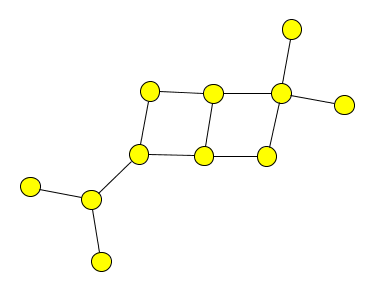
\includegraphics[scale=1.0]{simple.png}
	\caption{A simple graph}
	\label{simple_graphml}
\end{figure}
\end{center}


And corresponded graphml file showed in the Listing~\ref{simple_graphml_file}

\begin{center}
\begin{lstlisting} [language=xml, tabsize=2, caption={Simple graphml file},label=simple_graphml_file]
<graphml>
  <graph id="G" edgedefault="undirected">
    <node id="n0"/>
    <node id="n1"/>
    <node id="n2"/>
    <node id="n3"/>
    <node id="n4"/>
    <node id="n5"/>
    <node id="n6"/>
    <node id="n7"/>
    <node id="n8"/>
    <node id="n9"/>
    <node id="n10"/>
    <edge source="n0" target="n2"/>
    <edge source="n1" target="n2"/>
    <edge source="n2" target="n3"/>
    <edge source="n3" target="n5"/>
    <edge source="n3" target="n4"/>
    <edge source="n4" target="n6"/>
    <edge source="n6" target="n5"/>
    <edge source="n5" target="n7"/>
    <edge source="n6" target="n8"/>
    <edge source="n8" target="n7"/>
    <edge source="n8" target="n9"/>
    <edge source="n8" target="n10"/>
  </graph>
</graphml>
\end{lstlisting}
\end{center}

\subsubsection{DOT graph file format}
"DOT is a plain text graph description language. It is a simple way of describing graphs that both humans and computer programs can use. DOT graphs are typically files that end with the .gv (or .dot) extension.


At its simplest, DOT can be used to describe an undirected graph. An undirected graph shows simple relations between objects, such as friendship between people. The graph keyword is used to begin a new graph, and nodes are described within curly braces. A double-hyphen (\textendash \textendash) is used to show relations between the nodes."~\cite{DOT}

\begin{center}
\begin{lstlisting} [language=C, tabsize=2, caption={DOT file format: undirected graph}]
graph graphname {
     a - - b - - c;
     b - - d;
}
\end{lstlisting}
\end{center}

"Similar to undirected graphs, DOT can describe directed graphs, such as flowcharts and dependency trees. The syntax is the same as for undirected graphs, except the digraph keyword is used to begin the graph, and an arrow ($->$) is used to show relationships between nodes."~\cite{DOT}

\begin{center}
\begin{lstlisting} [language=C, tabsize=2, caption={DOT file format: directed graph}]
graph graphname {
     a -> b -> c;
     b -> d;
}
\end{lstlisting}
\end{center}

Visual representation of both graphs showed in the Figure~\ref{dot_graphs} below.

\begin{figure}
\begin{center}
    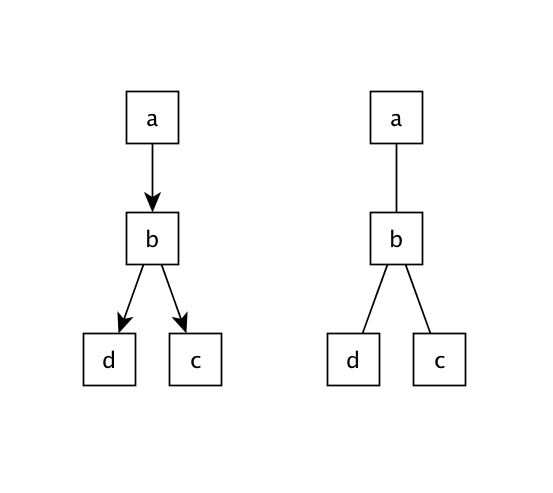
\includegraphics[scale=0.3]{dot_graph.png}
	\caption{Directed and undirected graphs}
	\label{dot_graphs}
\end{center}
\end{figure}

\subsubsection{DGML}
DGML is an XML-based file format for directed graphs. Here is what a simple directed graph with three nodes and two links between them looks like

\begin{center}
\begin{lstlisting} [language=XML, tabsize=2, caption={DGML file format}]
<?xml version='1.0' encoding='utf-8'?>
<DirectedGraph xmlns="http://schemas.microsoft.com/vs/2009/dgml">
  <Nodes>
    <Node Id="a" Label="a" Size="10" />
    <Node Id="b" Background="#FF008080" Label="b" />
    <Node Id="c" Label="c" Start="2010-06-10" />
  </Nodes>
  <Links>
    <Link Source="a" Target="b" />
    <Link Source="a" Target="c" />
  </Links>
  <Properties>
    <Property Id="Background" Label="Background" DataType="Brush" />
    <Property Id="Label" Label="Label" DataType="String" />
    <Property Id="Size" DataType="String" />
    <Property Id="Start" DataType="DateTime" />
  </Properties>
</DirectedGraph>
\end{lstlisting}
\end{center}

The complete XSD schema for DGML is available at \url{http://schemas.microsoft.com/vs/2009/dgml/}. DGML not only allows describing nodes and links in a graph, but also annotating those nodes and links with any user defined property and/or category.

\subsubsection{GXL}
"GXL (Graph eXchange Language) is a standard format for exchanging graph-based data. It is the culmination of a cooperative effort among an international group of researchers from disparate areas, including software reengineering and graph transformation. Researchers and tool builders have had a growing interest in comparing and combining approaches to their respective problems and leveraging each other's results. These collaborations provide lessons learned that are critical to advancing the maturity of the discipline. A standard exchange format for data facilitates tool interoperability and allows them to use a "best of breed" approach when building a workbench.


Interoperability is the challenge of enabling tools from different suppliers to work together. Wasserman [1] describes a taxonomy with five types of interoperability: platform, presentation, data, control, and process. Another model from Earl has three levels: control, user interface, and data. Data interoperability appears in both of them.


Data interoperability requires the data to be compatible both syntactically and semantically. In other words, tools need to agree on both the format and the meaning of this data. The graph-based data model of GXL can be used to represent both instance data and schemas.


Thus, GXL provides a standardized notation for exchanging instance data (graphs) including their structure (graph schemas). Both instance and schema graphs are encoded using the same XML (eXtensible Markup Language) DTD (Document Type Definition). While these schema graphs do not provide semantics, they serve as a basis for users to agree upon semantics. This feature is important because it helps tools and researchers communicate about the assumptions inherent in their approaches. This increased mutual understanding is a critical step in building on each other's work to increase the impact of research results.


In addition to being a generic format for representing graph structures, GXL is also suitable for object-relational data. Consequently, GXL can be used to represent data from a wider range of applications, including as data repositories and fact bases from reengineering tools."~\cite{GXL}

\subsubsection{SVG}
"SVG has been in development since 1999 by a group of companies within the W3C after the competing standards Precision Graphics Markup Language (PGML) – developed from Adobe's PostScript – and Vector Markup Language (VML) – developed from Microsoft's RTF – were submitted to W3C in 1998. SVG drew on experience from the designs of both those formats.


SVG allows three types of graphic objects:
\begin{itemize}
\item Vector graphics
\item Raster graphics
\item Text
\end{itemize}

Graphical objects, including PNG and JPEG raster images, can be grouped, styled, transformed, and composited into previously rendered objects. SVG does not directly support z-indices[5] that separate drawing order from document order for overlapping objects, unlike some other vector mark up languages like VML. Text can be in any XML name space suitable to the application, which enhances search ability and accessibility of the SVG graphics. The feature set includes nested transformations, clipping paths, alpha masks, filter effects, template objects and extensibility.


Since 2001, the SVG specification has been updated to version 1.1 (current Recommendation) and 1.2 (still a Working Draft). The SVG Mobile Recommendation introduced two simplified profiles of SVG 1.1, SVG Basic and SVG Tiny, meant for devices with reduced computational and display capabilities. SVG Tiny later became an autonomous Recommendation (current version 1.2) and the basis for SVG 1.2. In addition to these variants and profiles, the SVG Print specification (still a Working Draft) contains guidelines for printable SVG 1.2 and SVG Tiny 1.2 documents.
The Canvas element in HTML 5 provides an approach to rendering dynamic graphics in HTML that's procedural rather than declarative: instead of specifying the shapes to draw in XML, the author executes drawing commands from a script. Canvas doesn't allow for static rendering, and drawn elements are not identifiable in a DOM-like way."~\cite{SVG}

\section{Solution}
\label{solution}

\subsection{Cluster Analysis Results Visualization}

As was discussed before in the Section~\ref{dataset_description} cluster analysis result graph is binary tree.

"A binary tree is a connected acyclic graph such that the degree of each vertex is no more than 3. A rooted binary tree is such a graph that has one of its vertices of degree no more than 2 singled out as the root. With the root thus chosen, each vertex will have a uniquely defined parent, and up to two children; however, so far there is insufficient information to distinguish a left or right child. If we drop the connectedness requirement, allowing multiple connected component in the graph, we call such a structure a forest"~\cite{BINARY_TREE} Simple binary tree showed on the Figure~\ref{simple_binary_tree}

\begin{figure}
\begin{center}
	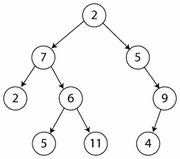
\includegraphics[scale=1.0]{simple_binary_tree.png}
	\caption{A simple binary tree graph}
	\label{simple_binary_tree}
\end{center}
\end{figure}


There several visualization methods for binary trees and more specific methods for cluster result. The main method for visualizing clusters is - dendrogram. Here is sample dendrogram visualization on the Figure~\ref{dendrogram_1} produced by MATLAB 7.2.

\begin{figure}
\begin{center}
	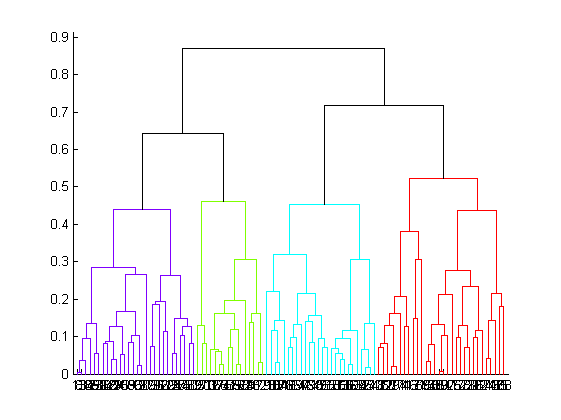
\includegraphics[scale=1.0]{dendrogram.png}
	\caption{Dendrogram}
	\label{dendrogram_1}
\end{center}
\end{figure}


The Figure~\cite{polardendrogram} shows polar dendrogram visualization algorithm of the same cluster tree produced by MATLAB.

\begin{figure}
\begin{center}
	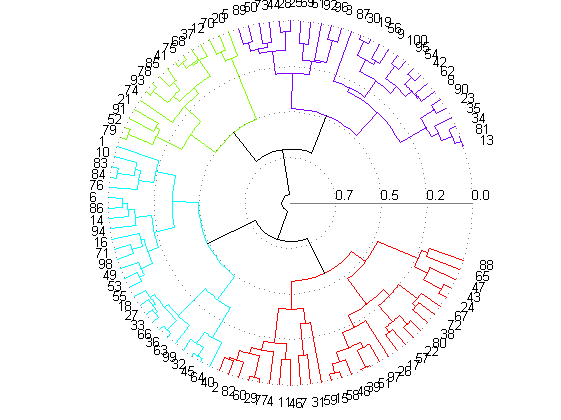
\includegraphics[scale=1.0]{polardendrogram.png}
	\caption{Polar Dendrogram}
	\label{polardendrogram}
\end{center}
\end{figure}

One of the main ideas was to use polar dendrogram algorithm for cluster visualization. The Figure~\cite{JUNG_radial_layout} shows visualization of the Cluster using native JUNG radial layout algorithm. Red are nodes and white is edges, black is background. As picture shows algorithm doesn't count nature of the cluster - very deep binary tree not wide as it is common for cluster analysis results, that's why it has many edge everlappings.


\begin{figure}
\begin{center}
	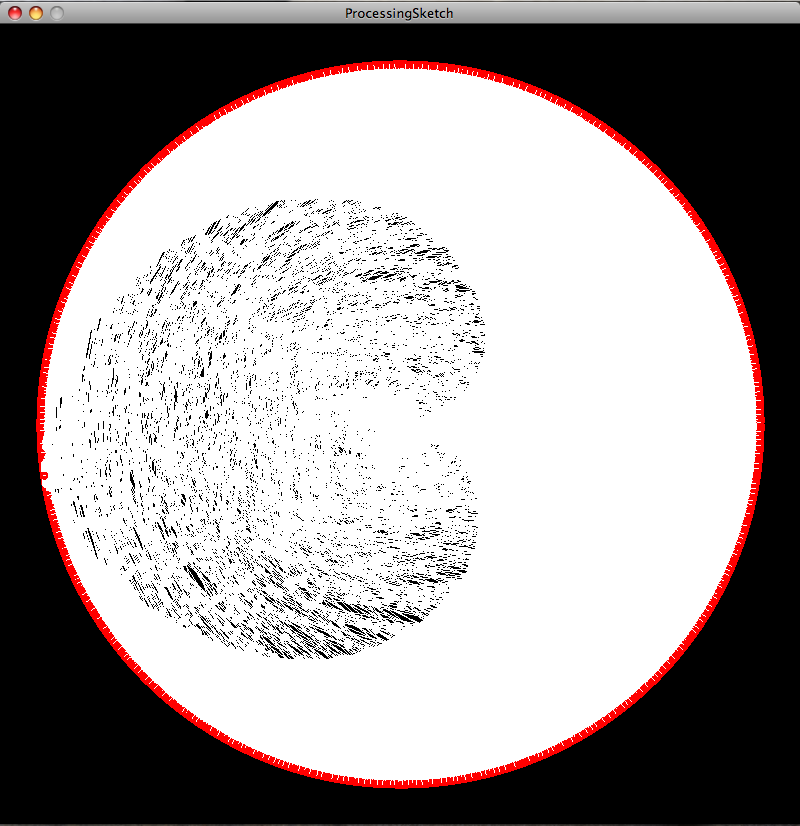
\includegraphics[scale=0.3]{using_JUNG_radial.png}
	\caption{Cluster visualization using JUNG radial layout}
	\label{JUNG_radial_layout}
\end{center}
\end{figure}


Also to visualization issue it has performance issue -- without any measurement was seen for an eye that program does not allow smooth interaction. Low performance issue was in nature of the visualization in the JUNG: it uses very complex hierarchical structure with many utility classes per visualized object and the cost is big memory usage. Also JUNG uses Java 2D~\cite{JAVA_2D} which by itself is "heavyweight" because it's part of the Java AWT -- Abstract Windows Toolkit.


"The Abstract Window Toolkit (AWT) is Java's original platform-independent windowing, graphics, and user-interface widget toolkit. The AWT is now part of the Java Foundation Classes (JFC) — the standard API for providing a graphical user interface (GUI) for a Java program. When Sun Microsystems first released Java in 1995, AWT widgets provided a thin level of abstraction over the underlying native user interface. For example, creating an AWT check box would cause AWT directly to call the underlying native subroutine that created a check box."~\cite{JAVA_AWT} This technology is outdated and replaced by Swing.


"Swing is the primary Java GUI widget toolkit. It is part of Sun Microsystems' Java Foundation Classes (JFC) — an API for providing a graphical user interface (GUI) for Java programs.
Swing was developed to provide a more sophisticated set of GUI components than the earlier Abstract Window Toolkit. Swing provides a native look and feel that emulates the look and feel of several platforms, and also supports a pluggable look and feel that allows applications to have a look and feel unrelated to the underlying platform."~\cite{JAVA_SWING}


"Since early versions of Java, a portion of the Abstract Window Toolkit (AWT) has provided platform-independent APIs for user interface components. In AWT, each component is rendered and controlled by a native peer component specific to the underlying windowing system.
By contrast, Swing components are often described as lightweight because they do not require allocation of native resources in the operating system's windowing toolkit. The AWT components are referred to as heavyweight components."~\cite{JAVA_SWING} More detail comparison can be found here.~\cite{AWT_VS_SWING}


The Figure~\ref{cluster_jogl_impl} shows improved JUNG radial algorithm and own visualization implementation using JOGL. JOGL will be discussed in the Section~\ref{opengl}.


\begin{figure}
\begin{center}
	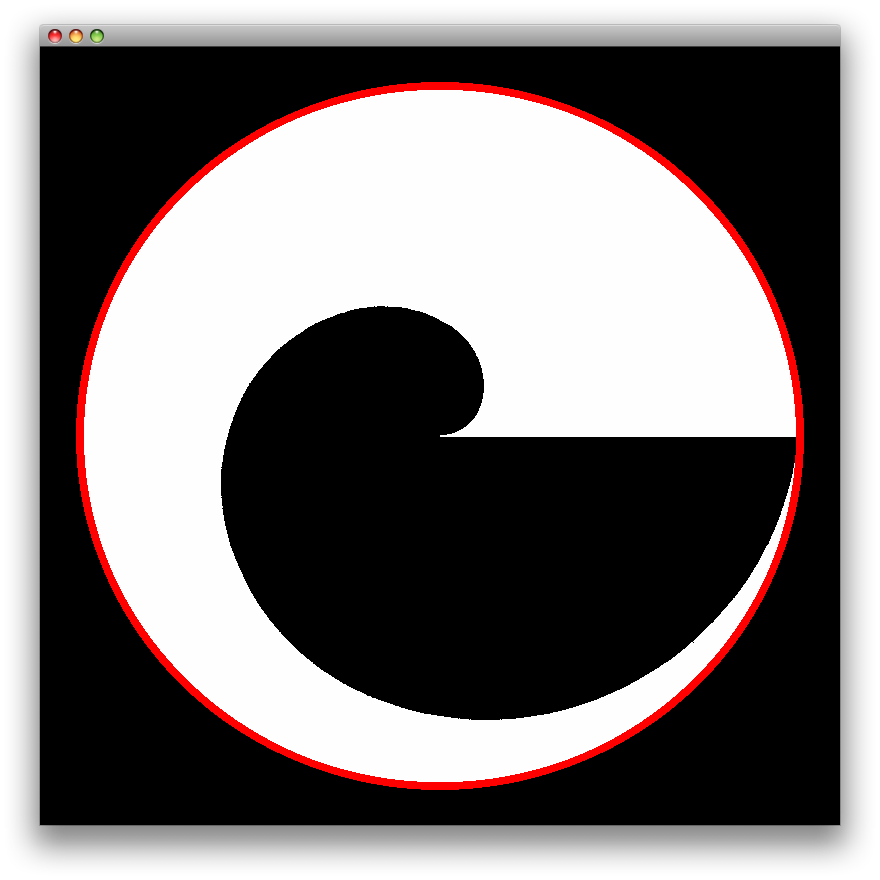
\includegraphics[scale=0.3]{cluster_jogl_impl.png}
	\caption{Cluster visualization using JOGL and improved JUNG radial layout}
	\label{cluster_jogl_impl}
\end{center}
\end{figure}


The Figure~\ref{cluster_jogl_impl_with_subgraph_1} and Figure~\ref{cluster_jogl_impl_with_subgraph_2} shows cluster visualization and highlighted subgraph using algorithm that was discussed in the Section~\ref{problem_statement_and_goal}. This pictures show the nature of the dataset. Improved version has good performance and better visualization but still has issues. Too many elements are in the scene, it is impossible to identify separate gene and trace highlighted graph genes.

\begin{figure}
\begin{center}
	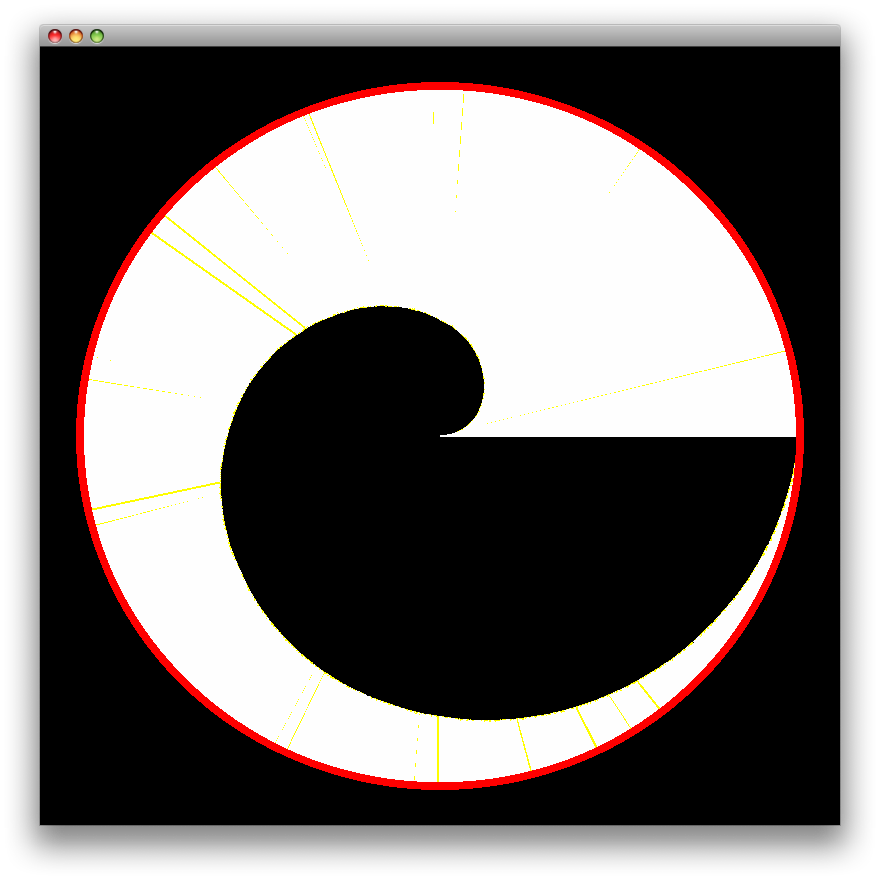
\includegraphics[scale=0.3]{cluster_jogl_impl_with_subgraph_1.png}
	\caption{Cluster graph and highlighted subgraph}
	\label{cluster_jogl_impl_with_subgraph_1}
\end{center}
\end{figure}

\begin{figure}
\begin{center}
	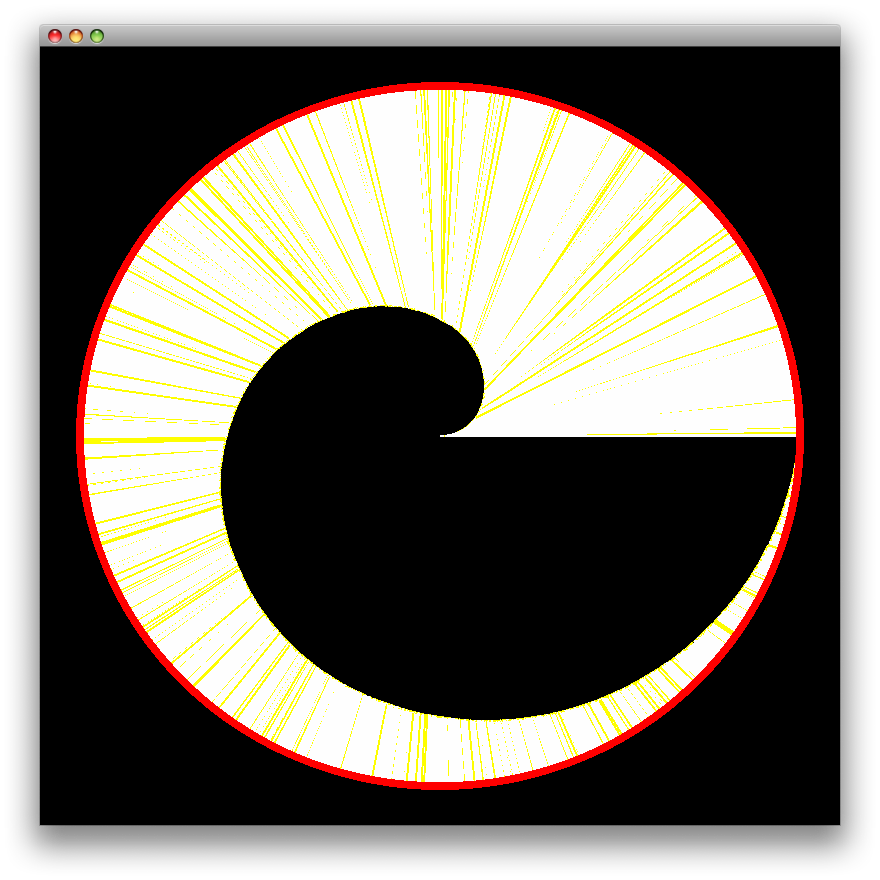
\includegraphics[scale=0.3]{cluster_jogl_impl_with_subgraph_2.png}
	\caption{Cluster graph and highlighted subgraph}
	\label{cluster_jogl_impl_with_subgraph_2}
\end{center}
\end{figure}


\subsection{Gene Ontology Visualization}

\section{Implementation}
\label{implementation}
Main language and platform for developing thesis is Java. "Java is a programming language and computing platform first released by Sun Microsystems in 1995. It is the underlying technology that powers state-of-the-art programs including utilities, games, and business applications. Java runs on more than 850 million personal computers worldwide, and on billions of devices worldwide, including mobile and TV devices."~\cite{java_com} Also, there are a lot of different libraries in Java. Every "common" part of the system could be replaceable. In the future sections would be detailed overview libraries for graphs, graph visualizations and graphic libraries.


Java is flexible platform which has big amount of different libraries. It helps not to write twice things already made but flexibility cause project structure complexity and library management. On the early stage there are no problems to control project throw sophisticated IDE (integrated development environment) but as project complexity grows more powerful building tool need appears. Maven is used during thesis work. 


Maven~\cite{MAVEN_HOME_PAGE} is free, open-source and de facto project management standard on the Java platform, is part of Apache software project developed and supported by ASF (Apache Software Foundation)~\cite{APACHE_FOUNDATION_HOME_PAGE}. "Maven provides a comprehensive approach to managing software projects. From compilation, to distribution, to documentation, to team collaboration, Maven provides the necessary abstractions that encourage reuse and take much of the work out of project builds."~\cite{MAVEN_BOOK_1}


"Maven is a project management framework, but this doesn't tell you much about Maven. It's the most obvious three-word definition of Maven the authors could come up with, but the term project management framework is a meaningless abstraction that doesn't do justice to the richness and complexity of Maven. Too often technologists rely on abstract phrases to capture complex topics in three or four words, and with repetition phrases such as project management and enterprise software start to lose concrete meaning.


When someone wants to know what Maven is, they will usually ask “What exactly is Maven?”, and they expect a short, sound-bite answer. “Well it is a build tool or a scripting framework” Maven is more than three boring, uninspiring words. It is a combination of ideas, standards, and software, and it is impossible to distill the definition of Maven to simply digested sound-bites. Revolutionary ideas are often difficult to convey with words. If you are interested in a fuller, richer definition of Maven read this introduction; it will prime you for the concepts that are to follow.


If Maven isn't a “project management framework". what is it? Here's one attempt at a description: Maven is a set of standards, a repository format, and a piece of software used to manage and describe projects. It defines a standard life cycle for building, testing, and deploying project artifacts. It provides a framework that enables easy reuse of common build logic for all projects following Maven's standards. The Maven project at the Apache Software Foundation is an open source community which produces software tools that understand a common declarative Project Object Model (POM). This book focuses on the core tool produced by the Maven project, Maven 2, a framework that greatly simplifies the process of managing a software project.


You may have been expecting a more straightforward answer. Perhaps you picked up this book because someone told you that Maven is a build tool. Don't worry, Maven can be the build tool you are looking for, and many developers who have approached Maven as another build tool have come away with a finely tuned build system. While you are free to use Maven as “just another build tool”, to view it in such limited terms is akin to saying that a web browser is nothing more than a tool that reads hypertext.


Maven and the technologies related to the Maven project are beginning to have a transformative effect on the Java community.
In addition to solving straightforward, first-order problems such as simplifying builds, documentation, distribution, and the deployment process, Maven also brings with it some compelling second-order benefits.


As more and more projects and products adopt Maven as a foundation for project management, it becomes easier to build relationships between projects and to build systems that navigate and report on these relationships. Maven's standard formats enable a sort of "Semantic Web" for programming projects. Maven's standards and central repository have defined a new naming system for projects. Using Maven has made it easier to add external dependencies and publish your own components.


So to answer the original question: Maven is many things to many people. It is a set of standards and an approach as much as it is a piece of software. It is a way of approaching a set of software as a collection of interdependent components which can be described in a common format. It is the next step in the evolution of how individuals and organizations collaborate to create software systems. Once you get up to speed on the fundamentals of Maven, you will wonder how you ever developed without it."~\cite{MAVEN_BOOK_2}


Maven's primary goal is to allow a developer to comprehend the complete state of a development effort in the shortest period of time. In order to attain this goal there are several areas of concern that Maven attempts to deal with:
\begin{itemize}
	\item making the build process easy
	\item providing a uniform build system
	\item providing quality project information
	\item providing guidelines for best practices development	
	\item allowing transparent migration to new features	
\end{itemize}


On the Figure~\ref{THESIS_FOLDER_STRUCTURE} showed structure of thesis project folder. Project uses stardard Maven project folder format. 


Here is overview of key parts: java source code stored in the "src/main/java" folder, tests source code stored in the "src/test/java. Necessary resources such as log4j configuration file stored in the "src/main/resources", in the same folder thesis properties file is stored. During "package" phase all resources are copied by Maven. 


"Native" directory stores JOGL native libraries to different platform such as Linux, Windows and Mac OS X. In the "lib.zip" stored jars for JUNG library which should be manually placed in the local Maven repository because they do not  exist in central Maven repository. All other dependencies are exist in Maven repositories and handled by default dependency process.


Complete builds are stored in the "build" folder. Latest build stored in the "build/latest" folder, other builds stored in the folder that has such name pattern:\texttt{GoClusterViz-\%version\%-\%build date\%-\%build time\%}. Each build folder contains corresponded native build for each of three platforms Linux, Windows and Mac OS X.


Cluster graph and Gene Ontology graphs stored in the "data" folder.

\begin{figure}
\begin{center}
	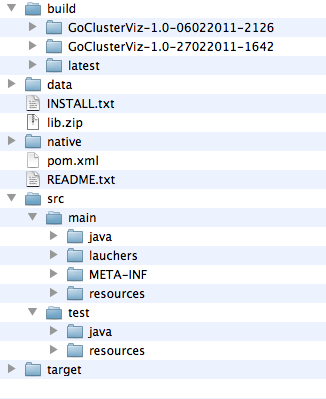
\includegraphics[scale=0.6]{thesis_folder_structure.png}
	\caption{Thesis folder structure}
	\label{THESIS_FOLDER_STRUCTURE}
\end{center}
\end{figure}

Second necessary part of the normal development process is revision control. "Revision control, also known as version control or source control (and an aspect of software configuration management or SCM), is the management of changes to documents, programs, and other information stored as computer files. It is most commonly used in software development, where a team of people may change the same files. Changes are usually identified by a number or letter code, termed the "revision number", "revision level", or simply "revision". For example, an initial set of files is "revision 1". When the first change is made, the resulting set is "revision 2", and so on. Each revision is associated with a timestamp and the person making the change. Revisions can be compared, restored, and with some types of files, merged."~\cite{REVISION_CONTROL} 


During thesis development was used Git version control system. "Git is a distributed revision control system with an emphasis on speed. Git was initially designed and developed by Linus Torvalds for Linux kernel development. Every Git working directory is a full-fledged repository with complete history and full revision tracking capabilities, not dependent on network access or a central server. Git's current software maintenance is overseen by Junio Hamano. Git is free software distributed under the terms of the GNU General Public License version 2. after he claimed that Andrew Tridgell had reverse-engineered the BitKeeper protocols.)
Torvalds wanted a distributed system that he could use like BitKeeper, but none of the available free systems met his needs, particularly his performance needs."~\cite{GIT} Git allows to store and work local on machine but for more safety reasons all source code stored on GitHub. GitHub is a web-based hosting service for software development projects that use the Git revision control system. GitHub provides free hosting open-source project. Thesis project home page on GitHub is \url{http://github.com/vadyalex/thesis} and source code url is \url{git://github.com/vadyalex/thesis.git} 

\begin{figure}
\begin{center}
	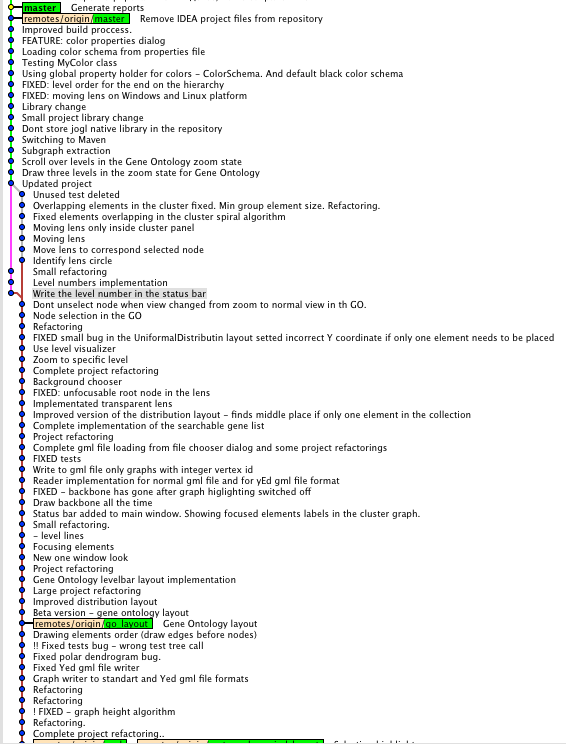
\includegraphics[scale=0.6]{commit_graph_gitk.png}
	\caption{Commit graph of the local repository made by gitk tool}
\end{center}
\end{figure}


\subsection{Java Graph Libraries Overview}


There are overview of a few libraries for working with graphs in Java

\begin{enumerate}

\item
Java Graph Editing Framework (GEF)~\cite{GEF}

The aim of project consists in generation of library for graph editing, which can be used for construction of high-end (high-quality) custom applications for working with graphs. 
GEF facilities (opportunities):
\begin{itemize}
	\item simple and clear design, which allows a developer to expand library's functionality 
	\item Node-Port-Edge model of graph's presentation, which permits to perform overwhelming majority of tasks occurring in working with graphs applications
	\item future XML-based format support (SVG)
\end{itemize}

\item
ILOG JViews ~\cite{ILOG_Jview}

ILOG JViews gives (grants) components, aimed for using in custom applications, and also in common with Ajax and Eclipse platform.

\item
JGraphT~\cite{JGraphT}

JGraphT is open source library, which provides with mathematical tool of graphs theory. JGraphT supports different kinds of graphs, including: oriented and unoriented graphs, graphs with weighted/non weighted/nominate (named) or anything else arc format, appointed 	by user, non upgradeable graphs - supported access to internal graphs in "Read Only" mode. Listenable graphs: allows outer listener to trace events appearance; sub graphs: graphs which are a view about other graphs. Being a powerful feature, JGraphT has been 	developed as easy and type-safe (with Java code generators use) feature for working with 	graphs. For example, any object can be node of a graph. You can build graphics on basis of: line, URL, XML documents and so forth, you can even build graphs of graphs.

\item
Java Universal Network / Graph Framework (JUNG)~\cite{JUNG}

"JUNG — the Java Universal Network/Graph Framework--is a software library that provides a common and extendible language for the modeling, analysis, and visualization of data that can be represented as a graph or network. It is written in Java, which allows JUNG-based applications to make use of the extensive built-in capabilities of the Java API, as well as those of other existing third-party Java libraries.


The JUNG architecture is designed to support a variety of representations of entities and their relations, such as directed and undirected graphs, multi-modal graphs, graphs with parallel edges, and hypergraphs. It provides a mechanism for annotating graphs, entities, and relations with metadata. This facilitates the creation of analytic tools for complex data sets that can examine the relations between entities as well as the metadata attached to each entity and relation.
The current distribution of JUNG includes implementations of a number of algorithms from graph theory, data mining, and social network analysis, such as routines for clustering, decomposition, optimization, random graph generation, statistical analysis, and calculation of network distances, flows, and importance measures (centrality, PageRank, HITS, etc.).


JUNG also provides a visualization framework that makes it easy to construct tools for the interactive exploration of network data. Users can use one of the layout algorithms provided, or use the framework to create their own custom layouts. In addition, filtering mechanisms are provided which allow users to focus their attention, or their algorithms, on specific portions of the graph.


As an open-source library, JUNG provides a common framework for graph/network analysis and visualization. We hope that JUNG will make it easier for those who work with relational data to make use of one anothers' development efforts, and thus avoid continually re-inventing the wheel."~\cite{JUNG_OVERVIEW}


JUNG library is widely used in differ amount of projects. Here is a list of projects using JUNG:

\begin{itemize}

\item ExtC: an Eclipse plug-in that is useful for locating large, noncohesive classes and for recommending how to split them into smaller, more cohesive classes. (Keith Cassell)~\cite{EXTC}

\item Djinn: a tool for visualizing java artifacts dependencies in a project: jars, directories, packages, classes. (Fabien Benoit)~\cite{DJINN}

\item Angur: An XML visualization/WYSWYG Editor (Amir Mohammad shahi)~\cite{ANGUR}

\item RDF Gravity: a tool for visualizing RDF/OWL graphs/ontologies. (Sunil Goyal, Rupert Westenthaler)~\cite{RDF_GRAVITY}

\item GUESS from HP Labs is a database-driven network analysis tool that provides flexible visualizations, scripting capabilities with Python/Jython, and interfaces with JUNG to let users take advantage of its algorithm library. (Eytan Adar, David Feinberg)~\cite{GUESS}

\item ADAPTNet is an applet that visualises the families of short oligo microarray probesets associated through common gene transcripts. (Michal Okoniewski, Tim Yates)~\cite{ADAPTNET}

\item Augur~\cite{AUGUR} is a visualization tool designed to support the distributed software development process. (Jon Froehlich)~\cite{AUGUR_2}

\item Ariadne is an Eclipse plug-in (under development) that links technical and social dependencies. (Cleidson de Souza et al.)~\cite{ARIADNE}

\item Netsight is a proof-of-concept tool for the visual exploratory data analysis of large-scale network and relational data sets. (Yan-Biao Boey, Joshua O'Madadhain, Scott White, Padhraic Smyth)~\cite{NETSIGHT}

\item InfoVis CyberInfrastructure provides an unified architecture in which diverse data analysis, modeling and visualization algorithms can be plugged in and run.~\cite{INFOVIS_CYBERINFRASTRUCTURE}

\item PWComp is a graph comparative metabolic pathway tool. (Joshua Adelman, Josh England, Alex Chen)~\cite{PWCOMP}

\item Google Cartography, featured in Google Hacks, uses the Google Search API to build a visual representation of the interconnectivity of streets in an area. (Richard Jones)~\cite{GOOGLE_CARTOGRAPHY}

\item GINY is a project with similar aims to that of JUNG, which contains some code derived from JUNG. (Rowan Christmas)~\cite{GINY}

\item GraphExplore is a JAVA application that renders networks of objects in a graphical form, which uses modified forms of the JUNG layout algorithm implementations. (Quanli Wang)~\cite{GRAPHEXPLORER}

\item TOTEM (TOolbox for Traffic Engineering Methods) provides a framework where researchers can integrate their traffic engineering algorithms. These algorithms can therefore be applied on models of real networks. The TOTEM toolbox also gives network operators the opportunity to experiment the currently developed traffic engineering algorithms on their own network. Today, the TOTEM toolbox already federates a large set of traffic engineering algorithms published in the scientific literature. This project uses JUNG for the graphical representation of the network topology. (S. Balon, O. Delcourt, J. Lepropre and F. Skivee)~\cite{TOTEM}

\item D2K ("Data to Knowledge") is a visual programming environment for building complicated data mining applications; T2K is a library of D2K modules that implements sophisticated algorithms for text analysis. Each of these uses JUNG for network visualization.~\cite{D2K}

\item graphBuilder is an application that allows users to build network representations of relational databases and data files. It has been designed as a tool for exploring online scientific data repositories. (Ben Raymond)~\cite{GRAPHBUILDER}

\item Semiophore is an application for exploring large graphs where there are many variables on both nodes and links (including time-based/event variables). It works with a relationnal database. It provides several visualization approaches. One of them is based on JUNG. It provides several analysis routines, featuring SNA measures among them. User can interact with the network : dynamic multi-variables filtering, dynamic aggregation, network editing and production of quicktime videos from longitudinal analysis are possible. Semiophore can handle text/XML documents with NLP information extraction and text summarization routines [English and French support only] in order to automatically build network maps of actors/information.~\cite{SEMIOPHORE}

\item Xholon uses JUNG to represent and visualize networks such as biochemical pathways and models (screenshots). (Ken Webb)~\cite{XHOLON}

\item Flink is a website presenting the social networks and research activity of Semantic Web researchers based on a number of sources (web pages, publication databases, email archives, FOAF data). Flink uses JUNG for network representation and visualization as well as for computing network measures. Flink has won 1st prize at the Semantic Web Challenge~\cite{SWC} of 2004. (Peter Mika)~\cite{FLINK}

\item T-Prox(approve sites) is a proxy, designed to be used for usability analyzes of websites. It uses JUNG to visualize the users path through the site. (Sven Lilienthal)~\cite{T_PROX}

\item Simple C-K Editor is a visualisation tool built on the C-K Design Theory. Its main purpose is to provide an easy tool to create, manipulate, edit and print C-K diagrams.~\cite{SIMPLE_C_K_EDITOR}

\item PCOPGene is web-based application to analise microarray data with large sample-series. The user can identify several kinds of non-linear expression relationships inside the gene network, study the expression dependence fluctuations in detail, and crossing the results with external biomedical data-servers.~\cite{PCOPGENE}

\end{itemize}

\end{enumerate}

There are a lot more graph visualization frameworks for Java: Piccolo~\cite{Piccolo}, The Visualization Toolkit (VTK)~\cite{VTK}, The InfoVis Toolkit~\cite{InfoVis_Toolkit}, Improvise~\cite{Improvise}. All of them can be used as for storing and visualizing graphs and networks. 


In the scope of current thesis work was used JUNG graph library to store graph structures.
	
\subsection{OpenGL visualization standart}
\label{opengl}
"OpenGL is a software interface to graphics hardware. This interface consists of about 120 distinct commands, which you use to specify the objects and operations needed to produce interactive three-dimensional applications.


OpenGL is designed to work efficiently even if the computer that displays the graphics you create isn't the computer that runs your graphics program. This might be the case if you work in a networked computer environment where many computers are connected to one another by wires capable of carrying digital data. In this situation, the computer on which your program runs and issues OpenGL drawing commands is called the client, and the computer that receives those commands and performs the drawing is called the server. The format for transmitting OpenGL commands (called the protocol) from the client to the server is always the same, so OpenGL programs can work across a network even if the client and server are different kinds of computers. If an OpenGL program isn't running across a network, then there's only one computer, and it is both the client and the server.


OpenGL is designed as a streamlined, hardware-independent interface to be implemented on many different hardware platforms. To achieve these qualities, no commands for performing windowing tasks or obtaining user input are included in OpenGL; instead, you must work through whatever windowing system controls the particular hardware you're using. Similarly, OpenGL doesn't provide high-level commands for describing models of three-dimensional objects. Such commands might allow you to specify relatively complicated shapes such as automobiles, parts of the body, airplanes, or molecules. With OpenGL, you must build up your desired model from a small set of geometric primitive - points, lines, and polygons."~\cite{THE_RED_BOOK}


There are many wrappers over OpenGL for developing on different programming languages. One of the favourite are JOGL and LWJGL.


"The Lightweight Java Game Library (LWJGL) is a solution aimed directly at professional and amateur Java programmers alike to enable commercial quality games to be written in Java. LWJGL provides developers access to high performance crossplatform libraries such as OpenGL (Open Graphics Library) and OpenAL (Open Audio Library) allowing for state of the art 3D games and 3D sound. Additionally LWJGL provides access to controllers such as Gamepads, Steering wheel and Joysticks. All in a simple and straight forward API.


LWJGL is not meant to make writing games particularly easy; it is primarily an enabling technology which allows developers to get at resources that are simply otherwise unavailable or poorly implemented on the existing Java platform. We anticipate that the LWJGL will, through evolution and extension, become the foundation for more complete game libraries and "game engines" as they have popularly become known, and hide some of the new evils we have had to expose in the APIs.


LWJGL is available under a BSD license, which means it's open source and freely available at no charge."~\cite{LWJGL}


In the thesis used JOGL wrapper library over OpenGL. "Java OpenGL (JOGL) is a wrapper library that allows OpenGL to be used in the Java programming language. It was originally developed by Kenneth Bradley Russell and Christopher John Kline, and was further developed by the Sun Microsystems Game Technology Group. As of 2010, it is an independent open source project under a BSD license. It is the reference implementation for Java Bindings for OpenGL (JSR-231).


The base OpenGL C API and associated operation system API, are accessed in JOGL via Java Native Interface (JNI) calls. As such, the underlying system must support OpenGL for JOGL to work. JOGL differs from some other Java OpenGL wrapper libraries in that it merely exposes the procedural OpenGL API via methods on a few classes, rather than trying to map OpenGL functionality onto the object-oriented programming paradigm. Indeed, most of the JOGL code is autogenerated from the OpenGL C header files via a conversion tool named GlueGen, which was programmed specifically to facilitate the creation of JOGL.


This design decision has both its advantages and disadvantages. The procedural and state machine nature of OpenGL is inconsistent with the typical method of programming under Java, which is bothersome to many programmers. However, the straightforward mapping of the OpenGL C API to Java methods makes conversion of existing C applications and example code much simpler. The thin layer of abstraction provided by JOGL makes runtime execution quite efficient, but accordingly is more difficult to code compared to higher-level abstraction libraries like Java3D. Because most of the code is autogenerated, changes to OpenGL can be rapidly added to JOGL."~\cite{JOGL}


\subsection{IO layer Implementation}

\subsection{Gene Ontology Visualization Implementation}
\subsection{Cluster Visualization Implementation}
	
\section{Conclusions}
\subsection{Future work}
\subsection{Problems during thesis work}

\section*{Glossary}
\addcontentsline{toc}{section}{Glossary}
GO -- Gene Ontology\\
XML -- eXtensible Markup Language\\
GML -- Graph Modelling Language\\
SVG -- Scalable Vector Graphics\\
IDE - Integrated Development Environment \\
JUNG -- Java Universal Network / Graph Framework\\
JOGL -- Java OpenGL\\
JNI -- Java Native API\\
LWJGL -- Lightweight Java Game Library\\

\addcontentsline{toc}{section}{References}
\begin{thebibliography}{99}

\mywebref{Biology}{Biotech}{http://biotech.icmb.utexas.edu/pages/bioinfo.html}
\mywebref{Bioinformatic}{Information about Bioinformatics}{http://www.absoluteastronomy.com/topics/Bioinformatics}
\mywebref{GO_website}{Gene Ontology}{http://www.geneontology.org/}
\mywebref{OBO}{The Open Biomedical Ontologies}{http://www.obofoundry.org/}

\bibitem{data_clustering_book}
G. Gan, C. Ma and J. Wu, Data Clustering. Theory, Algorithms, and Applications, Society for Industrial and Applied Mathematics pp 3, 2007.

\mywebref{Kerren}{Prof. Dr. Andreas Kerren home page}{http://w3.msi.vxu.se/users/akemsi/}
\mywebref{Schreiber}{Prof. Dr. Falk Schreiber home page}{http://bic-gh.ipk-gatersleben.de/~schreibe/}
\mywebref{ISOVIS}{ISOVIS research group home page}{http://cs.lnu.se/isovis/}
\mywebref{PBG}{Plant Bioinformatic research Group home page}{http://nwg.bic-gh.de/}
\mywebref{Graphlet}{Graphlet}{http://www.fmi.uni-passau.de/Graphlet/}
\mywebref{GML}{GML}{http://www.infosun.fim.uni-passau.de/Graphlet/GML/gml-tr.html}
\mywebref{GML_wiki}{GML supported programs}{http://en.wikipedia.org/wiki/Graph_Modelling_Language}
\mywebref{yEd}{yEd}{http://www.yworks.com/en/products_yed_about.html}
\mywebref{clairlib}{Clairlib}{http://www.clairlib.org/}
\mywebref{Cytoscape}{Cytoscape}{http://en.wikipedia.org/wiki/Cytoscape}
\mywebref{NetworkX}{NetworkX}{http://en.wikipedia.org/wiki/NetworkX}
\mywebref{ocamlgraph}{ocamlgraph}{http://ocamlgraph.lri.fr/}
\mywebref{OGDF}{OGDF}{http://www.ogdf.net/}
\mywebref{Tulip}{Tulip}{http://tulip.labri.fr/TulipDrupal/}
\mywebref{GraphML}{GraphML specification}{http://graphml.graphdrawing.org/}
\mywebref{GXL}{GXL introduction}{http://www.gupro.de/GXL/Introduction/section1.html}
\mywebref{SVG}{SVG information}{http://en.wikipedia.org/wiki/Scalable_Vector_Graphics}
\mywebref{GDC}{Graph Drawing Conference '95}{www.informatik.uni-trier.de/~ley/db/conf/gd/gd95.html}

%\mywebref{Radial_dendrogram}{Radial Dendrogram}{cs.sunysb.edu/~vislab/papers}
%\mywebref{Dendrogram}{Introduction into Dengrograms}{en.wikipedia.org/wiki/Dendrogram}

%\bibitem{Barlow_Neville}
T. Barlow and P. Neville, A comparison of 2D visualization of hierarchies, Information Visualization pp 131-138, 2001.

%\bibitem{Kreussler_Schumann}
M. Kreussler and H. Schumann, A flexible approach for visual data mining, IEEE Trans. VisualGraphics, vol. 8, no. 1, pp. 39-51, 2002.

%\bibitem{Yang_Ward}
J. Yang, M. Ward, and E. Rundensteiner, InterRing: An interactive tool for visually navigating and manipulatiung hierarchical structures, IEEE 2002 Symposium on Information Visualization, pp. 77-92, 2002.

\mywebref{java_com}{Java FAQ}{http://www.java.com/en/download/faq/whatis_java.xml}

\mywebref{BINARY_TREE}{Binary Tree definition}{http://www.wordiq.com/definition/Binary_tree}

\mywebref{JAVA_2D}{Java 2D reference}{http://java.sun.com/products/java-media/2D/reference/index.html}

\mywebref{JAVA_AWT}{Java AWT overview}{http://en.wikipedia.org/wiki/Abstract_Window_Toolkit}

\mywebref{JAVA_SWING}{Java SWING overview}{http://en.wikipedia.org/wiki/Swing_(Java)}

\mywebref{AWT_VS_SWING}{AWT vs SWING comparison}{http://edn.embarcadero.com/article/26970}

\mywebref{MAVEN_HOME_PAGE}{Maven project home page}{http://maven.apache.org/}

\mywebref{APACHE_FOUNDATION_HOME_PAGE}{Apache Foundation home page}{http://www.apache.org/}

\bibitem{MAVEN_BOOK_1}
Vincent Massol, Jason van Zyl, Better builds with Maven, Mergere Library Press, pp. 16, 2006.

\bibitem{MAVEN_BOOK_1}
Vincent Massol, Jason van Zyl, Better builds with Maven, Mergere Library Press, pp. 18, 2006.

\mywebref{REVISION_CONTROL}{Revision Control definition}{http://en.wikipedia.org/wiki/Revision_control}

\mywebref{GIT}{Git overview}{http://en.wikipedia.org/wiki/Git_(software)}

\mywebref{}{}{}

\mywebref{GEF}{Java Graph Editing Framework}{http://gef.tigris.org/}

\mywebref{ILOG_Jview}{ILOG Jview}{http://www.ilog.com/products/jviews/}

\mywebref{JGraphT}{JGraphT)}{http://jgrapht.sourceforge.net/}

\mywebref{JUNG}{Java Universal Network / Graph Framework (JUNG)}{http://jung.sourceforge.net/}

\mywebref{JUNG_OVERVIEW}{JUNG graph library overview}{http://jung.sourceforge.net/index.html}

\mywebref{EXTC}{ExtC}{http://code.google.com/p/ext-c/}

\mywebref{DJINN}{Djinn}{http://www.jnovation.net/djinn}

\mywebref{ANGUR}{Angur}{http://angur.sourceforge.net/}

\mywebref{RDF_GRAVITY}{RDF Gravity}{http://semweb.salzburgresearch.at/apps/rdf-gravity/index.html}

\mywebref{GUESS}{GUESS}{http://www.hpl.hp.com/research/idl/projects/graphs/index.html}

\mywebref{ADAPTNET}{ADAPTNet}{http://bioinformatics.picr.man.ac.uk/adaptnet}

\mywebref{AUGUR}{Augur}{http://www.cs.washington.edu/homes/jfroehli/publications/GROUP2005_SeekingTheSource.pdf}

\mywebref{AUGUR_2}{Jon Froehlich web page}{http://www.cs.washington.edu/homes/jfroehli/}

\mywebref{ARIADNE}{Ariadne}{http://projects.ischool.washington.edu/mcdonald/cscw04/papers/desousa-cscw04.pdf}

\mywebref{NETSIGHT}{Netsight}{http://jung.sourceforge.net/netsight}

\mywebref{INFOVIS_CYBERINFRASTRUCTURE} {InfoVis CuberInfrastructure}{http://iv.slis.indiana.edu/sw/}

\mywebref{PWCOMP}{PWComp}{http://www.ocf.berkeley.edu/\~Ejadelman/pwcomp/}

\mywebref{GOOGLE_CARTOGRAPHY}{Google Cartography}{http://richard.jones.name/google-hacks/google-cartography/google-cartography.html}

\mywebref{GINY}{GINY}{http://csbi.sourceforge.net/}

\mywebref{GRAPHEXPLORER}{GraphExplorer}{http://graphexplore.cgt.duke.edu/}

\mywebref{TOTEM}{TOTEM}{http://totem.run.montefiore.ulg.ac.be/}

\mywebref{D2K}{D2K}{http://alg.ncsa.uiuc.edu/do/downloads}

\mywebref{GRAPHBUILDER}{graphBuilder}{http://aadc-maps.aad.gov.au/analysis/gb.cfm}

\mywebref{SEMIOPHORE}{Semiophore}{http://www.semiophore.net/}

\mywebref{XHOLON}{Xholon}{http://sourceforge.net/projects/xholon/}

\mywebref{FLINK}{Flink}{http://flink.semanticweb.org/}

\mywebref{SWC}{Semantic Web Challenge}{http://challenge.semanticweb.org/}

\mywebref{T_PROX}{T-Prox}{http://www.t-prox.net/}

\mywebref{SIMPLE_C_K_EDITOR}{Simple C-K Editor}{http://code.google.com/p/ckeditor}

\mywebref{PCOPGENE}{PCOPGene}{http://revolutionresearch.uab.es/}

\bibitem{THE_RED_BOOK}
Dave Shreiner, Mason Woo, Jackie Neider, Tom Davis, OpenGL(R) Programming Guide: The Official Guide to Learning OpenGL(R), Version 2.1 (6th Edition), Addison-Wesley Professional, 2007.

\mywebref{LWJGL}{LWJGL}{http://www.lwjgl.org/}

\mywebref{JOGL}{JOGL}{http://jogamp.org/}

\mywebref{Piccolo}{Piccolo}{http://www.cs.umd.edu/hcil/jazz/}

\mywebref{VTK}{Visualisation Toolkit}{http://www.vtk.org/}

\mywebref{InfoVis_Toolkit}{InfoVis Toolkit)}{http://ivtk.sourceforge.net/}

\mywebref{Improvise}{Improvise project homepage}{http://www.cs.ou.edu/~weaver/improvise/index.html}

\end{thebibliography}

\newpage
\section*{Appendix A: Listing of the complex gml file}
\addcontentsline{toc}{section}{Appendix A: Listing of the complex gml file}

\begin{center}
	\lstinputlisting[language=xml, tabsize=2, basicstyle=\footnotesize, numberstyle=\footnotesizefr]{YedGraph.gml}
\end{center}

\end{document}